% 
%  chapter7.tex
%  ISELthesis
%  
%  Created by Matilde Pós-de-Mina Pato on 2012/10/09.
%
\chapter{Evaluation}
\label{cha:evaluation}

This chapter evaluates the prototype described in Chapter~\ref{cha:impl} and answers the two
research questions of Section~\ref{sec:int_objectives}: whether internal function calls are bound
correctly at deployment time on both providers (RQ1), and how much that resolution costs (RQ2).

\section{Scope and Goals}
\label{sec:eval-scope}

Both the correctness checks and the measurements exercise only \emph{local} operations:
constructing a workflow model, traversing it, resolving internal calls against the registry,
reading and writing the registry file, and packaging a Lambda bundle. Operations that call the
cloud provider (Lambda/IAM/S3 requests, Cloud Run/Cloud Functions APIs, the QuickFaaS subprocess)
are deliberately excluded, for two reasons. First, they are dominated by network and
provider-side latency, and that cost is already known: deploying a workflow and the functions it
calls, whether with the two tools used separately or through this integration, takes minutes,
most of it spent by the provider building and activating each function. Timing it again would
measure the provider rather than the integration. Second, these operations are non-deterministic
and out of the unit-test scope by design. The correctness checks replace them with test doubles.
For RQ2, the evaluation therefore isolates what the integration adds: \emph{how much local work
does the unification layer add to a deployment, how does it scale with the number of calls and
the size of the registry, and how many requests does it send to the provider?} The first two
parts are measured, and the third is counted from the implementation
(Section~\ref{sec:eval-api-calls}).

Section~\ref{sec:eval-correctness} addresses RQ1. Sections~\ref{sec:eval-resolution}
to~\ref{sec:eval-api-calls} address RQ2, and are followed by a count of the manual steps the
integration removes (Section~\ref{sec:eval-manual-effort}) and by the packaging overhead of the
AWS provider (Section~\ref{sec:eval-bundle}).

\section{Correctness of the Resolution Ladder}
\label{sec:eval-correctness}

RQ1 asks whether the resolution ladder binds each internal call to the right endpoint and deploys
a function only when its absence is confirmed. Each production resolver
(\texttt{Aws\allowbreak Internal\allowbreak Function\allowbreak Resolver} and
\texttt{Workflow\allowbreak Internal\allowbreak Function\allowbreak Resolver}) has a unit-test
suite that resolves a small workflow in each situation the ladder can meet. The provider is
replaced by test doubles: a function lookup that answers ``found'', ``not found'' or ``access
denied'' per region, a fixed list of regions, and a deployer that records the deployments it is
asked for. The registry is a real file in a temporary directory. Each test checks the endpoint
written into the call, the registry contents afterwards and, where relevant, whether the deployer
was called or the resolution aborted.

Table~\ref{tab:eval-correctness} lists the situations with the behaviour that the ladder
semantics prescribe (Section~\ref{sec:walkthrough} and Section~\ref{subsec:validation-error-semantics}). The observed behaviour matches the
expected behaviour in every case: all 46 resolver tests (23 for AWS, 23 for GCP) pass, as do the
two tests of the registry bootstrap.

\begin{table}[htbp]
  \centering
  \caption{Situations covered by the resolver unit tests, with the expected behaviour. Each row is
  tested on both AWS and GCP unless marked otherwise. Every test passes.}
  \label{tab:eval-correctness}
  \begin{tabular}{|p{0.42\textwidth}|p{0.48\textwidth}|}
    \hline
    \textbf{Situation} & \textbf{Expected and observed behaviour} \\
    \hline
    Registry entry valid (Level~1) & call bound to the registered endpoint \\
    \hline
    Registry entry whose endpoint changed (drift) & registry updated; call bound to the current
    endpoint \\
    \hline
    Registry entry for a function no longer in its region (stale) & function searched in all
    regions; if found, the entry is replaced; otherwise the entry is removed and the resolution
    aborts \\
    \hline
    Validation of a registry entry denied by the provider & resolution aborts; entry kept \\
    \hline
    Not in the registry, found in one region (Level~2) & call bound; function registered \\
    \hline
    Found in several regions & resolution aborts (ambiguous name) \\
    \hline
    Explicit \texttt{region/name} reference & only that region is queried \\
    \hline
    Every candidate region inaccessible, function not found & resolution aborts with a distinct
    error \\
    \hline
    Not found anywhere, descriptor given (Level~3) & function deployed once from the descriptor;
    registered; call bound \\
    \hline
    Not found, some regions inaccessible, descriptor given & resolution aborts; nothing deployed \\
    \hline
    Not found anywhere, no descriptor given & resolution aborts; nothing deployed \\
    \hline
    Internal calls inside branches, iterations and parallel steps & all resolved (five tests) \\
    \hline
    External calls & host and path unchanged \\
    \hline
    Call setting both \texttt{internalFunction} and a literal \texttt{host}/\texttt{path} & rejected
    before the ladder starts \\
    \hline
    Internal call that declares a body (AWS only) & rejected before the ladder starts; nothing
    deployed (Section~\ref{sec:runtime-invocation}) \\
    \hline
    Several internal calls in one workflow & registry read once \\
    \hline
    Registry entry holding a \texttt{cloudfunctions.net} URL (GCP only) & validated against
    Cloud Run like any other hit; the live URL is bound (Section~\ref{subsec:gcp-cloud-run-functions}) \\
    \hline
    Registry file missing (provider-independent) & registry rebuilt from the provider's catalogue \\
    \hline
  \end{tabular}
\end{table}

\section{Methodology}
\label{sec:eval-methodology}

Benchmarks were implemented with the Java Microbenchmark Harness (JMH) 1.37, using
\texttt{Average\allowbreak Time} mode with results reported in microseconds per operation ($\mu$s/op). Each
measured value is consumed through a \texttt{Blackhole} to prevent dead-code elimination by the
JIT compiler. Every figure reported in this chapter was measured with three JVM forks, three
warm-up iterations and five measurement iterations of one second each
(\texttt{-f 3 -wi 3 -i 5 -w 1 -r 1}), so each value is the mean of fifteen measured iterations
across three JVMs, of already-JIT-compiled code. All experiments come from one run of the whole
suite except T6 and T7, the two experiments on the production resolvers, which were measured in
later sessions with the same settings on the same machine. Where the sessions can be compared,
they agree to within a few percent.

\paragraph{Caveat on absolute values.}
Measurements were taken on an Apple Silicon laptop running macOS, otherwise idle but not a
dedicated benchmarking machine. With three forks the run-to-run spread is small: the 99.9\%
confidence interval is under 1\% of the score for half the measurements and under 6\% for nine out
of ten. The tables omit those intervals for readability. The few points where the interval is a
large fraction of the score are identified in the text and should be read as noise. How far the
values carry over to other hardware is discussed in Section~\ref{sec:eval-threats}.

\paragraph{Experiment identifiers.}
Experiments keep the identifiers they carry in the benchmark suite: T1--T14 measure resolution
and the registry, and S1 measures packaging size.

\paragraph{Notation.}
Table~\ref{tab:eval-notation} lists the symbols the experiments share. What changes between
experiments is the \emph{relationship} among these quantities. The count of provider requests in
Section~\ref{sec:eval-api-calls} adds one more, $G$, defined there.

\begin{table}[htbp]
  \centering
  \caption{Notation used throughout the evaluation.}
  \label{tab:eval-notation}
  \begin{tabular}{|c|l|}
    \hline
    \textbf{Symbol} & \textbf{Meaning} \\
    \hline
    $N$ & total number of \texttt{call} steps in the workflow (internal or external), $N = I + E$ \\
    \hline
    $I$ & number of internal calls (repetitions counted) \\
    \hline
    $E$ & number of external calls (repetitions counted) \\
    \hline
    $R$ & number of entries in the registry file when it is read/written \\
    \hline
    $F$ & number of \emph{distinct} internal functions the workflow references \\
    \hline
    $K$ & number of successive registry writes (T8, T9) \\
    \hline
    $R_0$ & number of entries in the registry before the writes (T8, T9) \\
    \hline
  \end{tabular}
\end{table}

$R$ is the physical size of the registry file and is not the same as $F$: a registry may hold
$R{=}1000$ entries while a workflow references only $F{=}10$ of them. Internal calls are
distributed round-robin over the $F$ distinct functions.

\section{Resolution Overhead and Scalability}
\label{sec:eval-resolution}

\paragraph{Cost of the unification (T1).}
The first experiment isolates the cost of resolving an internal call against the cost of a call
that needs no resolution. It runs the single-read reference resolver over a workflow of $N$ calls
against a one-entry registry ($R{=}1$), once with every call internal and once with every call
external. Both variants pay one registry read, because the resolver reads the file before walking
the tree whether or not anything needs resolving. That read is what the $N{=}1$ figures measure,
about $9.8\,\mu$s (Table~\ref{tab:eval-t1} and Figure~\ref{fig:eval-t1}). The production deployers
do not pay it for a workflow without internal calls, because they skip resolution altogether. The
external column is therefore the baseline of the resolver, not the cost of deploying such a
workflow. What separates the two columns is the per-call work.
The internal path adds a lookup in the in-memory snapshot, the split of the resolved URL into host
and path, and the rebuilding of the call node, which together cost about $0.22\,\mu$s per call,
against about $0.006\,\mu$s for an external call, whose node is left unchanged. Resolving a 200-call
workflow therefore costs $54.9\,\mu$s, of which the single read is roughly a fifth. Because the
registry holds one entry, this experiment says nothing about the cost of reading a larger file,
which is the variable the next experiment isolates. The $N{=}10$ point is noise: its value,
$16.9 \pm 16.8\,\mu$s, has a confidence interval that reaches almost down to zero.

\begin{figure}[htbp]
  \centering
  {\captionsetup{textfont=sf}\captionof{table}{T1: resolution time ($\mu$s) of a workflow of $N$ calls, all internal vs.\ all
  external, with $R{=}1$. Both columns include the one registry read the resolver always performs.}
  \label{tab:eval-t1}}
  \begin{minipage}[c]{0.31\textwidth}
    \centering
    \small
    \begin{tabular}{|r|r|r|}
      \hline
      \textbf{$N$} & \textbf{Internal} & \textbf{External} \\
      \hline
      1   & 10.1 & 9.8  \\
      \hline
      2   & 10.4 & 9.8  \\
      \hline
      5   & 11.1 & 9.8  \\
      \hline
      10  & 16.9 & 9.8  \\
      \hline
      20  & 14.5 & 9.8  \\
      \hline
      50  & 21.3 & 10.0 \\
      \hline
      100 & 32.2 & 10.3 \\
      \hline
      200 & 54.9 & 10.9 \\
      \hline
    \end{tabular}
  \end{minipage}\hfill
  \begin{minipage}[c]{0.66\textwidth}
    \centering
    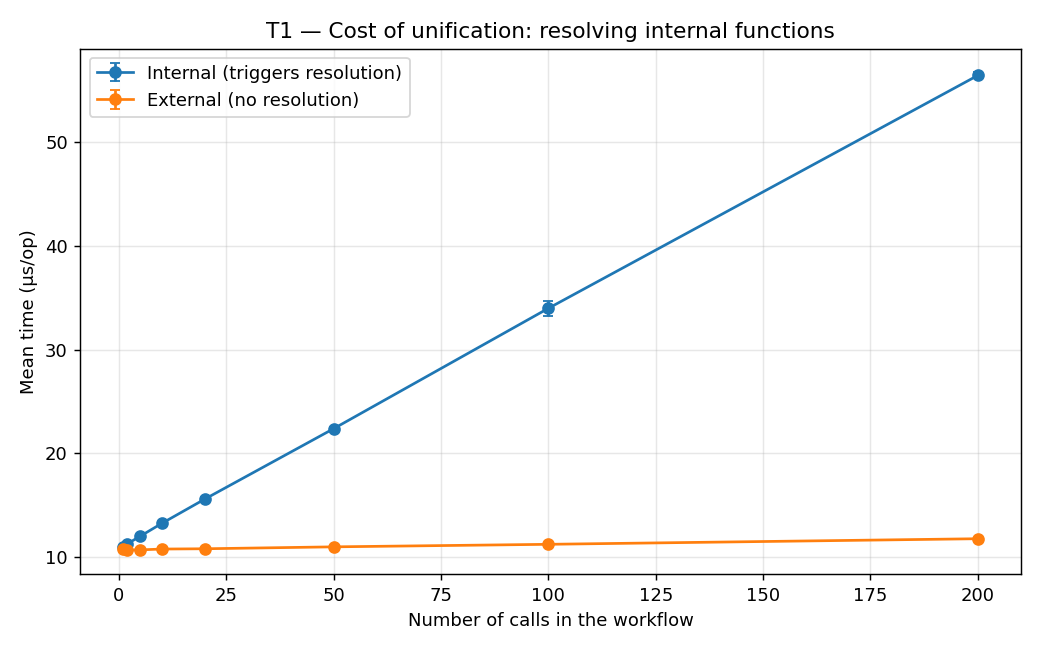
\includegraphics[width=\linewidth]{images/benchmarks/T1_resolution_overhead.png}
  \end{minipage}
  {\captionof{figure}{T1: resolution time of a workflow of $N$ calls, all internal against all external,
  with $R{=}1$. Both lines start from the one registry read the resolver always performs, and only
the internal line then grows with $N$. The error bar at $N{=}10$ reaches almost down to zero.}
  \label{fig:eval-t1}}
\end{figure}

\paragraph{Effect of registry size (T2).}
The second experiment varies the registry size. Unlike T1, it runs the naive reference resolver,
which re-reads and re-parses the whole registry file once for every internal call, so a workflow of
$N$ internal calls pays $N$ reads of an $R$-entry file. Table~\ref{tab:eval-t2} and
Figure~\ref{fig:eval-t2} divide each total by $N$, which gives the cost of one call and therefore of
one read. That cost grows with $R$ and is essentially independent of $N$: about $10.3\,\mu$s of
fixed I/O and parsing per read plus about $0.17\,\mu$s per registered entry. The four $N$ curves in
Figure~\ref{fig:eval-t2} collapse onto a single line, confirming that the total cost grows in direct
proportion to both the number of calls and the registry size. The two terms of that per-call cost
are equal when $0.17\,R = 10.3$, that is at $R \approx 60$: below that size the fixed cost of
opening and parsing the file dominates, and only
above it does the number of entries become the larger term. A registry holding the few dozen
functions of a realistic system therefore sits around or below that crossover, where the fixed cost
dominates, which is what makes reading it once per workflow (rather than once per call) the
change worth making.

\begin{figure}[htbp]
  \centering
  {\captionsetup{textfont=sf}\captionof{table}{T2: per-call resolution cost as a function of registry size $R$, with the registry
  re-read on every internal call: total time divided by $N$, averaged over $N \in \{1, 10, 50,
  200\}$.}
  \label{tab:eval-t2}}
  \begin{minipage}[c]{0.31\textwidth}
    \centering
    \small
    \begin{tabular}{|r|r|}
      \hline
      \textbf{$R$} & \textbf{Per call ($\mu$s)} \\
      \hline
      1    & 10.5  \\
      \hline
      10   & 11.9  \\
      \hline
      50   & 18.3  \\
      \hline
      200  & 44.5  \\
      \hline
      1000 & 183.4 \\
      \hline
    \end{tabular}
  \end{minipage}\hfill
  \begin{minipage}[c]{0.66\textwidth}
    \centering
    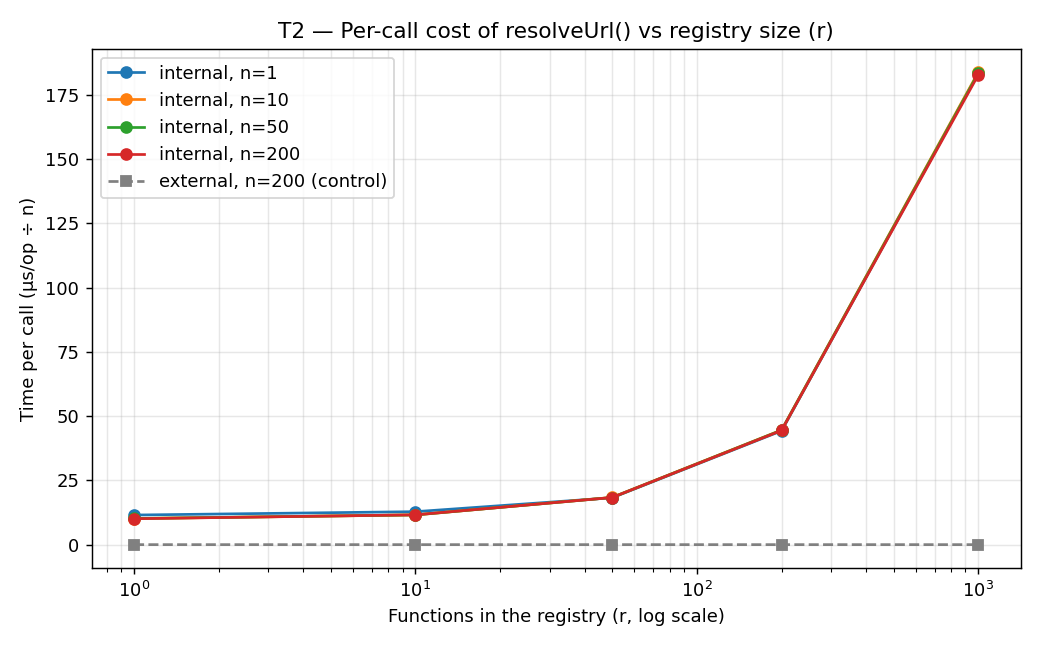
\includegraphics[width=\linewidth]{images/benchmarks/T2_registry_scaling.png}
  \end{minipage}
  {\captionof{figure}{T2: per-call resolution cost as a function of registry size $R$, for $N \in \{1, 10,
  50, 200\}$ internal calls. The external-call control does not read the registry.}
  \label{fig:eval-t2}}
\end{figure}

\paragraph{The single-read optimisation (T3).}
Reading the registry once per workflow into an in-memory snapshot and resolving against it
removes that product: the cost becomes one read proportional to the registry size plus a cheap
constant-time lookup per call. Table~\ref{tab:eval-t3} compares resolving the registry per call (naive) against a
single read per resolution (optimised). With the snapshot, the cost becomes almost independent of
$N$ (each row is flat to within a few tenths of a microsecond across a two-hundred-fold increase
in the number of calls) and reduces to the cost of one read of an $R$-entry file. The speedup
therefore grows with the product $N \cdot R$, reaching $200\times$ in the largest configuration measured
($N{=}200$, $R{=}1000$: $36.7$\,ms down to $0.18$\,ms).

\begin{figure}[htbp]
  \centering
  {\captionsetup{textfont=sf}\captionof{table}{T3: total resolution time ($\mu$s), naive (per-call read) vs.\ optimised (single
  read).}
  \label{tab:eval-t3}}
  \small
  \begin{tabular}{|l|r|r|r|r|}
    \hline
     & $N{=}1$ & $N{=}10$ & $N{=}50$ & $N{=}200$ \\
     \hline
    naive, $R{=}1$        & 9.8  & 98.0     & 492      & 1\,999    \\
    \hline
    optimised, $R{=}1$    & 10.0 & 10.0     & 10.1     & 10.3      \\
    \hline
    naive, $R{=}50$       & 17.9 & 180      & 901      & 3\,630    \\
    \hline
    optimised, $R{=}50$   & 18.4 & 18.3     & 18.5     & 18.5      \\
    \hline
    naive, $R{=}1000$     & 183  & 1\,839   & 9\,239   & 36\,670   \\
    \hline
    optimised, $R{=}1000$ & 182  & 183      & 182      & 184       \\
    \hline
  \end{tabular}
\end{figure}

\paragraph{Confirming the optimisation on real workflows (T4).}
T4 exercises the resolution of a real \texttt{Workflow} object, not the isolated store primitive,
across a grid of $1$ to $50$ distinct functions and $1$ to $200$ calls, with the registry always
hitting ($R{=}F$). The naive path is dominated by the number of calls, at roughly $10\,\mu$s per
call (one whole registry read each) and grows only mildly with $F$, since a larger $F$ means
a larger file to re-read (Table~\ref{tab:eval-t4-naive}). The optimised path pays that read once
and then about $0.22\,\mu$s per call, so $N$ still weighs more than $F$, but far less than on the
naive path (Table~\ref{tab:eval-t4-optimized}). At $F{=}1$ it goes from $10.2$ to $54.7\,\mu$s as $N$ goes from 1 to
200, where the naive path goes from $10.4$ to $2\,069\,\mu$s. At $N{=}1$ it goes only from
$10.2$ to $18.5\,\mu$s as $F$ goes from 1 to 50.
The speedup is therefore $1\times$ at $N{=}1$, where both paths read the file exactly once, and
climbs to $38\times$ ($F{=}1$) and $58\times$ ($F{=}50$) at $N{=}200$.

\begin{figure}[htbp]
  \centering
  \begin{minipage}[t]{0.48\textwidth}
    \centering
    {\captionsetup{textfont=sf}\captionof{table}{T4: naive resolution time ($\mu$s) of a real workflow, $F$ distinct functions vs.\
    $N$ calls, $R{=}F$.}
    \label{tab:eval-t4-naive}}
    \small
    \begin{tabular}{|r|r|r|r|r|r|}
      \hline
      $F\backslash N$ & 1 & 5 & 10 & 50 & 200 \\
      \hline
      1  & 10.4 & 52.3 & 105 & 525 & 2\,069 \\
      \hline
      2  & 10.8 & 53.0 & 106 & 534 & 2\,142 \\
      \hline
      5  & 11.1 & 53.9 & 108 & 543 & 2\,150 \\
      \hline
      10 & 11.6 & 58.5 & 116 & 582 & 2\,333 \\
      \hline
      20 & 13.3 & 66.6 & 133 & 665 & 2\,650 \\
      \hline
      50 & 18.7 & 92.5 & 185 & 929 & 3\,694 \\
      \hline
    \end{tabular}
  \end{minipage}\hfill
  \begin{minipage}[t]{0.48\textwidth}
    \centering
    {\captionsetup{textfont=sf}\captionof{table}{T4: optimised (single-read) resolution time ($\mu$s) of a real workflow, same grid
    as Table~\ref{tab:eval-t4-naive}.}
    \label{tab:eval-t4-optimized}}
    \small
    \begin{tabular}{|r|r|r|r|r|r|}
      \hline
      $F\backslash N$ & 1 & 5 & 10 & 50 & 200 \\
      \hline
      1  & 10.2 & 11.1 & 12.2 & 20.7 & 54.7 \\
      \hline
      2  & 10.4 & 11.2 & 12.2 & 21.1 & 54.1 \\
      \hline
      5  & 10.7 & 11.6 & 12.7 & 21.5 & 54.1 \\
      \hline
      10 & 11.5 & 12.7 & 13.8 & 22.5 & 55.8 \\
      \hline
      20 & 13.4 & 14.2 & 15.2 & 24.0 & 57.9 \\
      \hline
      50 & 18.5 & 19.4 & 20.8 & 29.4 & 63.3 \\
      \hline
    \end{tabular}
  \end{minipage}
\end{figure}

\paragraph{Registry size on a realistic workflow (T5).}
On a realistic workflow ($F{=}10$, $N{=}50$ fixed), T5 isolates the effect of the registry size.
Both paths grow with $R$, but for different reasons: the naive path re-reads the file on each of
the 50 calls, the optimised path reads it once, so the gap widens from $26\times$ at $R{=}10$ to
$46\times$ at $R{=}1000$ (Table~\ref{tab:eval-t5} and Figure~\ref{fig:eval-t5}). The optimised
column is the cost of one read plus 50 lookups, and tracks the per-read cost measured in T2.

\begin{figure}[htbp]
  \centering
  {\captionsetup{textfont=sf}\captionof{table}{T5: resolution time ($\mu$s) vs.\ registry size $R$, $F{=}10$/$N{=}50$ fixed.}
  \label{tab:eval-t5}}
  \begin{minipage}[c]{0.31\textwidth}
    \centering
    \small
    \setlength{\tabcolsep}{4pt}
    \begin{tabular}{|r|r|r|r|}
      \hline
      \textbf{$R$} & \textbf{naive} & \textbf{opt.} & \textbf{speedup} \\
      \hline
      10   & 589     & 22.6 & 26.1 \\
      \hline
      20   & 666     & 23.9 & 27.9 \\
      \hline
      50   & 930     & 29.3 & 31.8 \\
      \hline
      100  & 1\,378  & 37.8 & 36.5 \\
      \hline
      200  & 2\,246  & 54.9 & 40.9 \\
      \hline
      1000 & 9\,487  & 205  & 46.3 \\
      \hline
    \end{tabular}
  \end{minipage}\hfill
  \begin{minipage}[c]{0.66\textwidth}
    \centering
    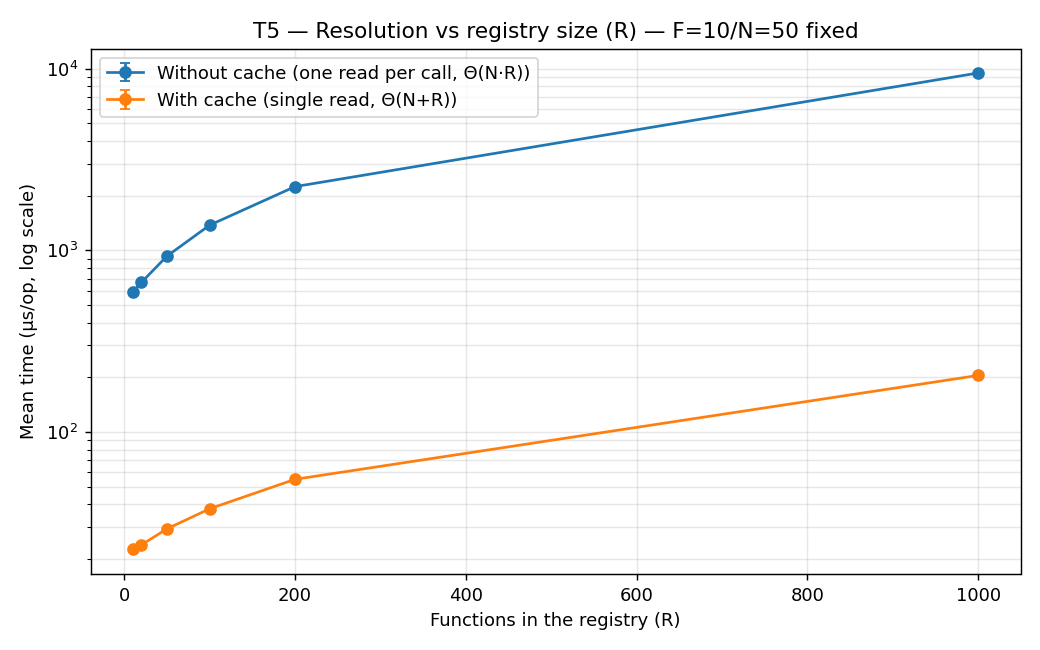
\includegraphics[width=\linewidth]{images/benchmarks/T5_resolution_by_registry.png}
  \end{minipage}
  {\captionof{figure}{T5: resolution time against registry size $R$ with $F{=}10$/$N{=}50$ fixed,
  per-call read against single read (logarithmic vertical axis). Both paths grow with $R$, and the
  gap between them widens with it.}
  \label{fig:eval-t5}}
\end{figure}

\section{Real Auto-Deploy Resolvers and Write Path}
\label{sec:eval-real-resolvers}

\paragraph{Production resolvers (T6, T7).}
Experiments T6 and T7 measure the resolvers that actually run during deployment, one per
provider: \texttt{Aws\allowbreak Internal\allowbreak Function\allowbreak Resolver} (Table~\ref{tab:eval-t6}) and
\texttt{Workflow\allowbreak Internal\allowbreak Function\allowbreak Resolver} (Table~\ref{tab:eval-t7}), with the
registry always hitting ($R{=}F$). Both use the single-read snapshot described in
Section~\ref{subsec:store-internals}, whose effect T3--T5 demonstrated on the reference resolver.
Neither experiment reaches a provider, but each stands in for it differently. On AWS the
inspector is a local fake that confirms every registered function. On GCP the real
\texttt{Cloud\allowbreak Run\allowbreak V2\allowbreak Service\allowbreak Inspector} validates every
hit, and only its HTTP client is replaced by one that answers each \texttt{services.get} locally
with the registered URL, so building the request, obtaining the token and parsing the JSON
response are measured, and only the network round-trip is not. What both measure is therefore the
local part of the ladder. The result has the same shape as the already-optimised reference
implementation: a cost that is one registry read plus a constant per call. Reading down the
$N{=}1$ column gives the read (plus, on GCP, one validation), which grows with $F$ because
$R{=}F$. Reading along a row gives the per-call work, $0.07$--$0.14\,\mu$s on AWS and about
$0.95\,\mu$s on GCP. Resolving a 200-call workflow against a registry of 10 functions costs
$29.1\,\mu$s on AWS and $199.1\,\mu$s on GCP.

The GCP resolver costs more per call because it parses the resolved URL into host and path, and
because its Cloud Run client builds a request and parses a response, work that T6's fake skips
entirely. The two experiments therefore do not stand in for the provider on equal terms. Either
way, the local work of a validation is at most about a microsecond per call, whereas the request it
prepares is a network round-trip to the provider (Section~\ref{sec:eval-api-calls}).

\begin{figure}[htbp]
  \centering
  {\captionsetup{textfont=sf}\captionof{table}{T6: AWS provider: resolution time ($\mu$s) of the real resolver
  (\texttt{Aws\allowbreak Internal\allowbreak Function\allowbreak Resolver}), $R{=}F$, with the
  single-read optimisation.}
  \label{tab:eval-t6}}
  \small
  \begin{tabular}{|l|r|r|r|r|r|}
    \hline
    $F\backslash N$ & 1 & 5 & 10 & 50 & 200 \\
    \hline
    1  & 9.9  & 10.3 & 10.9 & 13.8 & 24.6 \\
    \hline
    2  & 10.2 & 11.0 & 11.4 & 14.7 & 26.3 \\
    \hline
    5  & 11.0 & 11.2 & 11.7 & 15.3 & 27.6 \\
    \hline
    10 & 11.7 & 12.2 & 12.7 & 16.3 & 29.1 \\
    \hline
    20 & 14.4 & 14.8 & 14.4 & 19.7 & 34.5 \\
    \hline
    50 & 20.0 & 20.3 & 20.3 & 26.6 & 47.5 \\
    \hline
  \end{tabular}
\end{figure}

\begin{figure}[htbp]
  \centering
  {\captionsetup{textfont=sf}\captionof{table}{T7: GCP provider: resolution time ($\mu$s) of the real resolver
  (\texttt{Workflow\allowbreak Internal\allowbreak Function\allowbreak Resolver}), $R{=}F$, with
  the single-read optimisation and with every hit validated
  through a Cloud Run client answered locally.}
  \label{tab:eval-t7}}
  \small
  \begin{tabular}{|l|r|r|r|r|r|}
    \hline
    $F\backslash N$ & 1 & 5 & 10 & 50 & 200 \\
    \hline
    1  & 11.8 & 15.8 & 21.3 & 59.3 & 207.1 \\
    \hline
    2  & 12.1 & 16.4 & 21.3 & 61.3 & 209.1 \\
    \hline
    5  & 13.0 & 17.5 & 21.9 & 62.4 & 211.5 \\
    \hline
    10 & 15.1 & 18.4 & 23.1 & 60.2 & 199.1 \\
    \hline
    20 & 15.4 & 19.2 & 24.0 & 61.5 & 205.9 \\
    \hline
    50 & 21.9 & 25.6 & 30.6 & 67.5 & 209.0 \\
    \hline
  \end{tabular}
\end{figure}

\paragraph{Registry write path (T8, T9).}
Writing is more expensive than resolving. Every \texttt{put()} re-reads and rewrites the entire
registry file, so registering $K$ functions costs close to $K$ times one write, and one write costs
what it costs to rewrite a file of the current size (Table~\ref{tab:eval-t8}). Both factors are
visible. Across $K$, the cost per write is nearly constant (at $R_0{=}0$ it moves only from
$45.5$ to $59.1\,\mu$s between $K{=}1$ and $K{=}100$, the mild increase expected from a file that
has gained $K$ entries during the run), so the total is linear in $K$, not compounding. Across
$R_0$, the cost per write grows roughly in proportion to the file: about $45\,\mu$s on an empty
registry, $114\,\mu$s at $R_0{=}200$ and $490\,\mu$s at $R_0{=}1000$. The registry size is
therefore not a second-order term for writes as it is for reads: it multiplies the cost of every
write.

The miss-then-write pattern at the level of the store
(\texttt{tryResolveEntry} followed by \texttt{put}) adds between 26\% and 62\%
(Table~\ref{tab:eval-t9}), because \texttt{tryResolveEntry} reads the whole file once more before
the write rewrites it. The production resolvers do not pay this extra cost: they look every call up
in the snapshot with \texttt{tryResolveEntryIn}, so their writes cost what T8 measures. The extra cost grows with $R_0$ (about 30\% on an empty registry, about
60\% at $R_0{=}1000$), which is what an extra full read of a growing file predicts. One point
disagrees, $K{=}10$ at $R_0{=}10$, and its confidence interval ($\pm732\,\mu$s on a mean of
$874\,\mu$s) says it is noise rather than an effect.

\begin{figure}[htbp]
  \centering
  {\captionsetup{textfont=sf}\captionof{table}{T8: total write time ($\mu$s): $K$ successive \texttt{put} calls, initial registry
  size $R_0$.}
  \label{tab:eval-t8}}
  \small
  \begin{tabular}{|l|r|r|r|r|r|}
    \hline
    $K\backslash R_0$ & 0 & 10 & 50 & 200 & 1000 \\
    \hline
    1   & 45.5     & 48.2     & 63.8     & 114       & 490       \\
    \hline
    5   & 224      & 242      & 329      & 529       & 1\,945    \\
    \hline
    10  & 463      & 496      & 640      & 1\,041    & 3\,751    \\
    \hline
    50  & 2\,517   & 2\,706   & 3\,650   & 5\,363    & 17\,942   \\
    \hline
    100 & 5\,914   & 6\,693   & 7\,594   & 11\,515   & 36\,195   \\
    \hline
  \end{tabular}
\end{figure}

\begin{figure}[htbp]
  \centering
  {\captionsetup{textfont=sf}\captionof{table}{T9: total write time ($\mu$s): $K$ successive miss+\texttt{put} pairs, initial
  registry size $R_0$.}
  \label{tab:eval-t9}}
  \small
  \begin{tabular}{|l|r|r|r|r|r|}
    \hline
    $K\backslash R_0$ & 0 & 10 & 50 & 200 & 1000 \\
    \hline
    1   & 57.2     & 62.7     & 90.2     & 164       & 686       \\
    \hline
    5   & 298      & 323      & 427      & 769       & 2\,901    \\
    \hline
    10  & 597      & 874      & 973      & 1\,557    & 5\,751    \\
    \hline
    50  & 3\,265   & 3\,510   & 5\,051   & 8\,144    & 28\,694   \\
    \hline
    100 & 8\,369   & 8\,307   & 10\,516  & 17\,689   & 58\,572   \\
    \hline
  \end{tabular}
\end{figure}

\section{Match Strategy, Mixed Workflows, and Structure}
\label{sec:eval-secondary}

\paragraph{Exact vs.\ suffix match (T10).}
The suffix-match path (regional disambiguation) fails the exact lookup and scans the loaded map,
reintroducing a cost proportional to the registry size, but over an already-loaded map: the ratio
to exact match grows steadily from $1.28\times$ at $R{=}10$ to $1.95\times$ at $R{=}1000$, and
stays cheap in absolute terms: $391\,\mu$s for fifty suffix lookups over a thousand-entry
registry (Table~\ref{tab:eval-t10} and Figure~\ref{fig:eval-t10}).

\begin{figure}[htbp]
  \centering
  {\captionsetup{textfont=sf}\captionof{table}{T10: exact vs.\ suffix match ($\mu$s), $F{=}10$/$N{=}50$ fixed.}
  \label{tab:eval-t10}}
  \begin{minipage}[c]{0.31\textwidth}
    \centering
    \small
    \begin{tabular}{|r|r|r|r|}
      \hline
      \textbf{$R$} & \textbf{exact} & \textbf{suffix} & \textbf{ratio} \\
      \hline
      10   & 22.5 & 28.8 & 1.28 \\
      \hline
      20   & 24.2 & 32.6 & 1.35 \\
      \hline
      50   & 29.2 & 40.2 & 1.38 \\
      \hline
      100  & 38.2 & 58.9 & 1.54 \\
      \hline
      200  & 55.0 & 92.6 & 1.68 \\
      \hline
      1000 & 201  & 391  & 1.95 \\
      \hline
    \end{tabular}
  \end{minipage}\hfill
  \begin{minipage}[c]{0.66\textwidth}
    \centering
    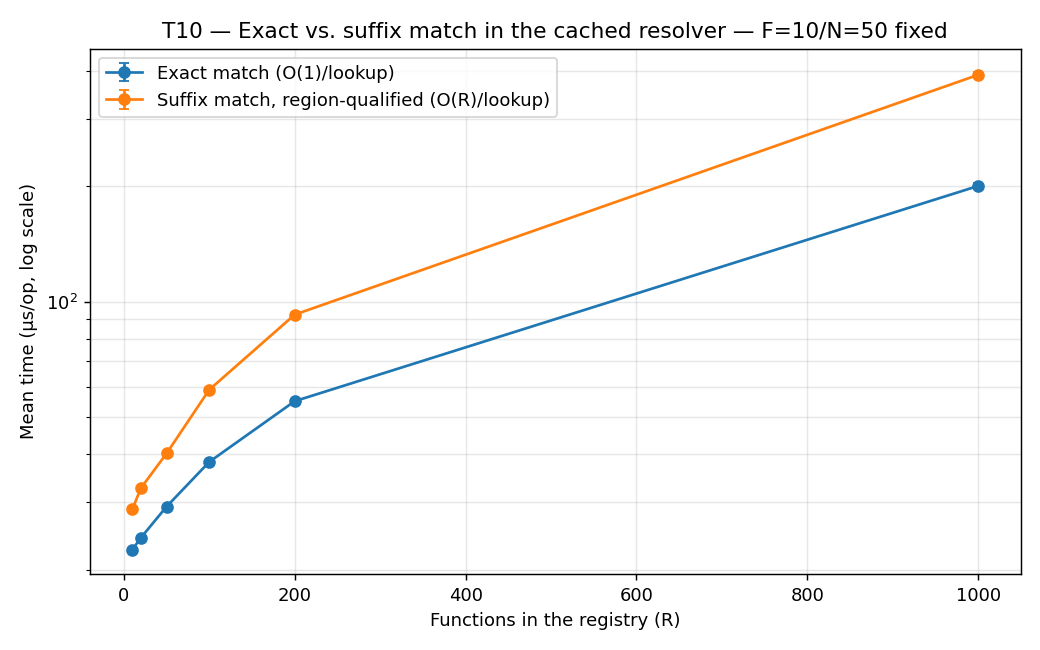
\includegraphics[width=\linewidth]{images/benchmarks/T10_resolution_key_match_strategy.png}
  \end{minipage}
  {\captionof{figure}{T10: exact against suffix match in the single-read resolver, $F{=}10$/$N{=}50$
  fixed (logarithmic vertical axis). Both grow with $R$ because of the read, and the suffix path adds
  a scan of the loaded map on top of it.}
  \label{fig:eval-t10}}
\end{figure}

\paragraph{Mixed internal/external workflows (T11, T12).}
Workflows that mix internal and external calls confirm that resolution cost scales with
$I$ (internal calls), not with $N{=}I{+}E$: the $I{=}0$ row stays at $11$--$14\,\mu$s as $E$ grows
to 200, because external calls incur no registry lookup, while reading down a column from $I{=}0$
to $I{=}200$ multiplies the cost by five (Table~\ref{tab:eval-t11}). Each row is flat apart from
isolated jumps of 16--22\% that vanish at the next point (at $E{=}10$ for $I{=}50$ and $I{=}200$,
and at $E{=}50$ for $I{\le}1$), and each column grows at about $0.22\,\mu$s per internal call, the same per-call figure as T1. The
registry-size effect shown in T5 is unchanged when a fraction of the calls are external: with
$I{=}40$ internal calls the cost still tracks the one read, from $20\,\mu$s at $R{=}10$ to
$199\,\mu$s at $R{=}1000$.

\begin{figure}[htbp]
  \centering
  {\captionsetup{textfont=sf}\captionof{table}{T11: resolution time ($\mu$s) of a mixed workflow with $I$ internal and
$E$ external calls, $R{=}F{=}10$ fixed.}
  \label{tab:eval-t11}}
  \small
  \begin{tabular}{|r|r|r|r|r|r|r|}
    \hline
    $I\backslash E$ & 0 & 1 & 5 & 10 & 50 & 200 \\
    \hline
    0   & 11.3 & 11.3 & 11.5 & 11.5 & 13.9 & 12.7 \\
    \hline
    1   & 11.5 & 11.7 & 11.8 & 11.8 & 14.4 & 12.7 \\
    \hline
    5   & 12.8 & 12.6 & 12.6 & 12.7 & 12.9 & 13.7 \\
    \hline
    10  & 13.7 & 13.8 & 13.8 & 13.8 & 14.0 & 14.7 \\
    \hline
    50  & 22.4 & 22.4 & 22.7 & 26.3 & 22.8 & 23.2 \\
    \hline
    200 & 55.8 & 55.9 & 56.2 & 67.1 & 57.4 & 56.8 \\
    \hline
  \end{tabular}
\end{figure}

\paragraph{Workflow shape (T13, T14).}
Nesting depth (T13) leaves the time essentially constant, $15.8$--$19.2\,\mu$s across depths 0--5
with 20 internal calls held fixed. The depth-2 point ($69.0 \pm 40.8\,\mu$s) is noise, as its own
confidence interval shows. Parallel width (T14) grows only with the total number of internal leaf
calls ($N = 5\times\text{width}$), at $0.22\,\mu$s per call (the same slope as the flat
workflows of T1 and T11), from $12.5\,\mu$s at $N{=}5$ to $119\,\mu$s at $N{=}500$
(Table~\ref{tab:eval-t14} and Figure~\ref{fig:eval-t14}). Although the resolver recurses explicitly into
\texttt{Iteration} and \texttt{Parallel} contexts, the shape of the tree is irrelevant: only the
count of internal calls matters.

\begin{figure}[htbp]
  \centering
  {\captionsetup{textfont=sf}\captionof{table}{T14: resolution time ($\mu$s) vs.\ \texttt{Parallel} branch width,
  $N = 5\times$ width, $R{=}F{=}10$.}
  \label{tab:eval-t14}}
  \begin{minipage}[c]{0.31\textwidth}
    \centering
    \small
    \begin{tabular}{|r|r|r|}
      \hline
      \textbf{Branches} & \textbf{$N$} & \textbf{Time ($\mu$s)} \\
      \hline
      1   & 5   & 12.5 \\
      \hline
      2   & 10  & 13.7 \\
      \hline
      5   & 25  & 17.0 \\
      \hline
      10  & 50  & 22.4 \\
      \hline
      20  & 100 & 33.2 \\
      \hline
      50  & 250 & 65.2 \\
      \hline
      100 & 500 & 119  \\
      \hline
    \end{tabular}
  \end{minipage}\hfill
  \begin{minipage}[c]{0.66\textwidth}
    \centering
    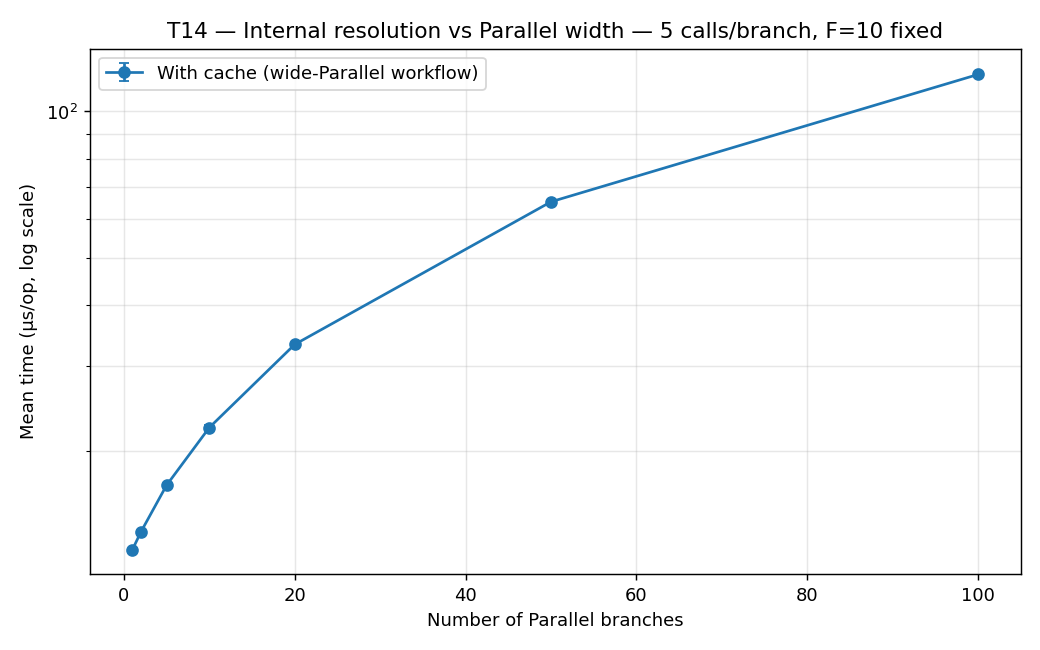
\includegraphics[width=\linewidth]{images/benchmarks/T14_internal_resolution_by_branch_width.png}
  \end{minipage}
  {\captionof{figure}{T14: resolution time against \texttt{Parallel} branch width, five internal calls per
  branch and $R{=}F{=}10$ fixed (logarithmic vertical axis). The time follows the total number of
  leaf calls $N = 5\times\text{width}$, not the shape of the tree.}
  \label{fig:eval-t14}}
\end{figure}

\FloatBlock

\section{Provider API Calls per Resolution}
\label{sec:eval-api-calls}

This section counts the network traffic the ladder generates, which the experiments above do not
see: the figures are read from the code of the two resolvers and of the clients they use, and they are
numbers of provider API requests, not latencies. Let $G$ be the number of candidate regions: the
regions enabled for the AWS account, or the Cloud Run locations visible to the GCP project.

\paragraph{What the count grows with.}
Both resolvers validate a registry hit on every internal \texttt{call} step, not once per distinct
function. The snapshot introduced in Section~\ref{sec:eval-real-resolvers} removes the repeated
\emph{file} reads, but it does not cache the live lookup that follows them. A workflow with
$I$ internal calls that all hit the registry therefore issues $I$ validation requests, even when
every call names the same function ($F{=}1$). Each is a network round-trip that T6 and T7 do not
include. The list of candidate regions, by contrast, is fetched at most once per deployment and
cached in the resolver, and a region scan is paid only by the calls that miss.

Table~\ref{tab:eval-api-calls} gives the count for each path through the ladder.

\begin{table}[htbp]
  \centering
  \caption{Provider API requests issued per internal call, by ladder path, counted from the
  implementation. $G$ is the number of candidate regions.}
  \label{tab:eval-api-calls}
  \begin{tabular}{|p{0.30\textwidth}|p{0.30\textwidth}|p{0.30\textwidth}|}
    \hline
    \textbf{Path} & \textbf{AWS} & \textbf{GCP} \\
    \hline
    Level~1, registry hit validated & 1 (\texttt{GetFunction} in the region taken from the stored
    ARN) & 1 (Cloud Run \texttt{services.get}) \\
    \hline
    Level~1, entry stale & 1 validation $+$ up to $G$ lookups (rediscovery) & 1 validation $+$ up
    to $G$ lookups \\
    \hline
    Level~2, bare \texttt{functionRef} & up to $G$ \texttt{GetFunction} (the scan stops at the
    second match) & up to $G$ \texttt{services.get} (likewise) \\
    \hline
    Level~2, \texttt{"region/name"} reference & 1 & 1 \\
    \hline
    Level~3, deployment & $G$ lookups (absence is confirmed in every region) $+$ the deployment
    below & $G$ lookups $+$ the deployment below \\
    \hline
  \end{tabular}
\end{table}

Two requests fall outside the per-call count. The candidate-region list costs one EC2
\texttt{Describe\allowbreak Regions} on AWS, and one Cloud Run \texttt{locations.list} request per response
page on GCP. The list is fetched lazily, so a deployment whose calls all resolve at Level~1 never pays
it. The registry bootstrap, which runs only when the registry file is absent and the workflow has
internal calls, costs that same region list plus one catalogue request per region and per response
page: \texttt{ListFunctions} on AWS, \texttt{services.list} on GCP.

\paragraph{The deployment itself (Level~3).}
A Level~3 deployment is the only path that writes to the provider, and it is dominated not by the
lookups above but by the deployment sequence described in
Sections~\ref{subsec:gcp-cloud-run-functions} and~\ref{subsec:omniflow-aws-deployer}: preparing
permissions, uploading and creating the function, and polling it until it is active. The polls
make the number of requests depend on how long the provider takes to activate the function, so
this path has no fixed count.

\paragraph{Consequence.}
For a deployment of $I$ internal calls, the traffic ranges from $I$ requests, when every call hits
a valid registry entry, to $1 + I \cdot G$ when the registry is empty and the references are bare
names. The registry is therefore not only a latency optimisation but the mechanism that keeps the
request count linear in $I$ instead of proportional to $I \cdot G$. A region-qualified reference
buys the same bound for a call that has to miss.

\section{Manual Effort Before and After}
\label{sec:eval-manual-effort}

The unification is meant to remove manual steps, so it is worth stating which ones, and counting
them. The comparison below is procedural, not a user study. It takes one task, making one
internal function available to one workflow on GCP, and follows it through the QuickFaaS
procedure of Section~\ref{subsec:quickfaas-example} and through the integrated procedure of
Section~\ref{sec:developer-workflow}. For each, it counts the developer actions required and the
values the developer has to carry by hand from one step to the next.

Table~\ref{tab:eval-manual-effort} lists the two sequences. What distinguishes them is not the
total amount of configuration, since the deployment descriptor is written either way, but the
hand-carried values. In the separate procedure, four values produced by one step are read by a
human and typed into the next: the OAuth client ID and secret into the authentication module, the
resulting \texttt{access\_token} into the descriptor, and the generated trigger URL into the
workflow definition. A typo in any of the first three stops the function from being deployed. A
typo in the URL is the costlier one, because it produces a workflow that deploys successfully and
fails only at run time. In the integrated procedure that number is zero: the access
token is taken from Application Default Credentials by the deployer, the invoker permission is
granted by the deployer, and the endpoint never leaves the tool: it goes from the provider into
the registry and from the registry into the rendered workflow.

\begin{table}[htbp]
  \centering
  \caption{Developer actions required to make one function available to one workflow on GCP.
  ``Carried by hand'' counts values produced by one step that the developer must read and re-enter
  in another.}
  \label{tab:eval-manual-effort}
  \begin{tabular}{|p{0.45\textwidth}|p{0.45\textwidth}|}
    \hline
    \textbf{QuickFaaS and OmniFlow used separately} & \textbf{Integrated (this work)} \\
    \hline
    Create an OAuth 2.0 client in the console and copy its client ID and secret \emph{(2 carried by
    hand)} & Not needed (the deployer uses Application Default Credentials, configured once per machine)
    \\
    \hline
    Run the auxiliary server, complete the OAuth flow, copy the \texttt{access\_token} into the
    descriptor \emph{(1 carried by hand)} & Not needed \\
    \hline
    Write \texttt{func-deployment.json} & Write \texttt{func-deployment.json} (same fields, without
    \texttt{accessToken}) \\
    \hline
    Write the cloud-agnostic function class & Write the cloud-agnostic function class \\
    \hline
    Run QuickFaaS to deploy the function & Not needed (the deployment is triggered by the workflow
    deployment, and only if the function is absent) \\
    \hline
    Grant the function public or invoker access in the console & Not needed (granted by the deployer) \\
    \hline
    Read the generated trigger URL from the console or terminal & Not needed \\
    \hline
    Write the workflow, pasting that URL as \texttt{host}/\texttt{path} \emph{(1 carried by hand)} &
    Write the workflow, naming the function:
    \texttt{internalFunction("name", "func-deployment.json")} \\
    \hline
    Run OmniFlow to deploy the workflow & Run OmniFlow to deploy the workflow \\
    \hline
    \textbf{9 steps, 4 values carried by hand} & \textbf{4 steps, 0 values carried by hand} \\
    \hline
  \end{tabular}
\end{table}

Two qualifications apply. First, the integrated procedure does not remove
configuration, it relocates it: the descriptor is still written by hand, and the credentials still
have to exist (Application Default Credentials on GCP, environment credentials on AWS), so
what is saved is the copying, not the setup. Second, the saving is per function and per endpoint
change, so it grows with the number of internal functions a workflow calls and with how often they
are redeployed. It is largest exactly where the manual procedure is most error-prone: a workflow
that calls several internal functions in several accounts (Chapter~\ref{cha:case-study}).

\section{Packaging Overhead (S1)}
\label{sec:eval-bundle}

The AWS provider added in this work packages a Lambda through the QuickFaaS provider-agnostic layer (the
developer hook plus the \texttt{AwsHttpTemplate} adapter and \texttt{aws-lambda-java-core}). Table
\ref{tab:eval-s1} compares the resulting bundle against an equivalent native \texttt{RequestHandler}
implementation of the same logic. The provider-agnostic layer adds about $0.9$\,KB (6.6\% of a trivial
bundle, and proportionally less for a function with real dependencies), consistent with the original QuickFaaS
evaluation for GCP and Azure~\cite{rodrigues2022quickfaas}.

\begin{table}[htbp]
  \centering
  \small
  \caption{S1: Lambda bundle size, provider-agnostic layer vs.\ native implementation.}
  \label{tab:eval-s1}
  \begin{tabular}{|l|r|}
    \hline
    \textbf{Bundle} & \textbf{Size} \\
    \hline
    Provider-agnostic (QuickFaaS hook + \texttt{AwsHttpTemplate} + \texttt{aws-lambda-java-core}) & 14\,552 bytes \\
    \hline
    AWS native (single \texttt{RequestHandler}, same logic) & 13\,647 bytes \\
    \hline
    \textbf{Delta (provider-agnostic layer overhead)} & \textbf{905 bytes} \\
    \hline
  \end{tabular}
\end{table}

\section{Discussion}
\label{sec:eval-discussion}

\paragraph{Answer to RQ1.}
In every situation of Table~\ref{tab:eval-correctness}, both resolvers take the expected decision:
each internal call is bound to the registered, current or discovered endpoint, and a function is
deployed only when it is in neither the registry nor any region and every region could be checked.
Stale entries that cannot be rediscovered, ambiguous names and inaccessible regions abort the
resolution instead of binding a call to a guess or deploying a duplicate. The answer to RQ1 is
therefore positive for the resolution logic on both providers, with one qualification: the
evidence comes from tests that simulate the provider.

\paragraph{Answer to RQ2.}
For RQ2, the benchmarks support five conclusions.

First, in the naive form the cost of the unification grows in direct proportion to both the
number of calls and the registry size, and is dominated by the fixed cost of reopening the
registry file up to $R \approx 60$ (Section~\ref{sec:eval-resolution}). Second, the single-read
optimisation eliminates that
call-times-registry-size product, reducing resolution to one read of the registry plus about
$0.22\,\mu$s per internal call, a speedup of $200\times$ in the largest configuration measured
(T3, T4, T5).
Third, the production resolvers (T6, T7) show the same one-read-plus-a-constant shape as the
optimised reference path: $29\,\mu$s (AWS) and $199\,\mu$s (GCP) for a 200-call workflow.
Fourth, resolution cost tracks
the number of internal calls rather than the workflow's total call count: external calls add only
the shared tree-traversal cost, never a registry lookup (T11, T12). Fifth, neither nesting depth
nor parallel width changes the cost beyond what the total count of internal calls already
predicts: the resolver's explicit recursion into \texttt{Iteration} and \texttt{Parallel} contexts
adds no measurable cost (T13, T14).

On the provider side, the request count of Section~\ref{sec:eval-api-calls} completes the answer:
resolution sends one request per internal call when every call hits a valid registry entry, and
up to one request per candidate region for each call that has to be discovered. The registry is
what keeps the common case at the lower bound.

\paragraph{Global framing.}
All measured values lie between microseconds and, in the worst write case, tens of milliseconds:
a hundred successive miss-and-register pairs against a thousand-entry registry (the most
expensive operation measured) cost $59$\,ms (T9). These figures are the local part of resolution
only, and a lower bound on its total cost: the network round-trips that validation and discovery
add are counted in Section~\ref{sec:eval-api-calls}, not timed (Section~\ref{sec:eval-scope}).
Endpoint resolution is nevertheless not the bottleneck of an integrated deployment: the dominant
cost is the cloud deployment itself, which takes minutes.

\section{Threats to Validity}
\label{sec:eval-threats}

The absolute numbers characterise the machine they were measured on
(Section~\ref{sec:eval-methodology}) rather than serverless deployment hardware in general. File I/O
dominates several of the experiments, so the factor they are most sensitive to is storage rather
than processor speed: on slower storage every registry read and write would cost more, while the
relationships between experiments would hold. What they support is therefore the shape of each
cost and the relationships between the experiments, which the shared measurement conditions make
comparable, rather than the values themselves. The individual points whose confidence intervals
are wide are identified where they appear and are not used to support any claim.

A second limit is one of provenance: because T6 and T7 come from later measurement sessions
(Section~\ref{sec:eval-methodology}), their comparison with the reference path of T4 should be read as
an order-of-magnitude comparison rather than an exact one.

The correctness evidence for RQ1 is mostly local. The resolver tests replace the provider with
test doubles, so they establish that each resolver takes the right decision given what the provider
reports, not that the real AWS and GCP APIs report what the doubles assume. The case study
(Section~\ref{sec:case-artifacts}) checks that assumption on GCP for one workflow, on the paths its
two deployments take: the registry bootstrap, Levels~2 and~3, and validated Level~1 hits. On AWS it
remains unchecked. Obtaining that evidence systematically means deploying workflows that contain
internal calls against real accounts on both providers, at each level of the ladder. This is listed
as future work (Section~\ref{sec:concl-future}).























































































